% !TeX program = lualatex

\documentclass[11pt]{article}
\usepackage[T1]{fontenc}
\usepackage{beramono}
\usepackage{listings}
\usepackage[usenames,dvipsnames]{xcolor}
\usepackage[mathletters]{ucs}
\usepackage[utf8x]{inputenc}
\usepackage{multirow}
\usepackage{multicol}
\usepackage{mathtools}
\usepackage{geometry}
\usepackage{siunitx}
\usepackage{float}
\usepackage{graphicx}
\usepackage{xcolor}
\usepackage{tikz}
\usetikzlibrary{patterns}
\geometry{margin=1.5in,top=1in,bottom=1in}

\newcommand{\pd}[2]{\frac{\partial #1}{\partial #2}}
\newcommand{\abs}[1]{\left|#1\right|}

\lstdefinelanguage{Julia}%
  {morekeywords={abstract,break,case,catch,const,continue,do,else,elseif,%
      end,export,false,for,function,immutable,import,importall,if,in,%
      macro,module,otherwise,quote,return,switch,true,try,type,typealias,%
      using,while},%
   sensitive=true,%
   alsoother={$},%
   morecomment=[l]\#,%
   morecomment=[n]{\#=}{=\#},%
   morestring=[s]{"}{"},%
   morestring=[m]{'}{'},%
}[keywords,comments,strings]%

\lstset{%
    language         = Julia,
    basicstyle       = \ttfamily,
    keywordstyle     = \bfseries\color{blue},
    stringstyle      = \color{magenta},
    commentstyle     = \color{ForestGreen},
    showstringspaces = false,
}

\title{\textbf{Final Report}}
\author{Pierce Hunter, Nick Kuckuck, Haoran Wang}
\date{7 June 2020}

\begin{document}
\maketitle
\section{1D Approach}
	We solved the 1D equation
	\begin{equation}
		\pd{^2u}{z^2} = -1; \quad 0\leq z\leq 1
	\end{equation}
	with boundary conditions
	\begin{equation}
		\pd{u}{z}\left(1\right) = 0; \quad u(0) = 0
	\end{equation}
	in the four following ways:
	\begin{itemize}
		\item Direct solve on the CPU
		\item CG on the CPU
		\item Direct solve on the GPU
		\item CG on the GPU.
	\end{itemize}
	For the one-dimensional problem we can utilize the straight-forward centered-difference discretization from class, namely
	\begin{equation}
		\frac{u_{j-1}-2u_j+u_{j+1}}{\Delta z^2} = -1 ~~\text{for}~~ 1\leq j\leq N.
	\end{equation}
	We discretize on the boundaries as well, giving the final system of equations
	\begin{equation}
		\begin{dcases}
		\frac{-2u_2 + u_3}{\Delta z^2} = -1\\
		\frac{u_{j-1}-2u_j+u_{j+1}}{\Delta z^2} = -1;& 3\leq j\leq N-1\\
		\frac{u_{N-1} - u_N}{\Delta z^2} = -1.
		\end{dcases}
	\end{equation}
	We can represent this system of equations as a matrix ($ A $) of the form
	\begin{equation}
		A = \frac{1}{\Delta z^2}\begin{bmatrix}
		-2&1&0&\cdots&0\\
		1&-2&1&\cdots&0\\
		\vdots&\ddots&\ddots&\ddots&\vdots\\
		0&\cdots&1&-2&1\\
		0&\cdots&0&1&-1
		\end{bmatrix}
	\end{equation}
	with the $ u $-column vector and $ b $-solution vector as
	\begin{equation}
		u = \begin{bmatrix}
		u_2\\
		\vdots\\
		u_N
		\end{bmatrix} \qquad b = \begin{bmatrix}
		-1\\\vdots\\-1
		\end{bmatrix}
	\end{equation}
	such that $ Au = b $.
	\section{2D Approach}
	We then expanded the problem to two-dimensions utilizing the same techniques. In 2D eq. (1) becomes
	\begin{equation}
		\pd{^2u}{y^2} + \pd{^2u}{z^2} = -1; \quad \begin{dcases}
		0\leq y\leq 1\\
		0\leq z\leq 1
		\end{dcases}
	\end{equation}
	and we expand the boundary conditions in (2) as
	\begin{align}
		\pd{u}{y} = 0&\text{ at }y=1\\
		\pd{u}{z} = 0&\text{ at }z=1\\
		u = 0&\text{ at }y=0\vphantom{\pd{u}{y}}\\
		u = 0&\text{ at }z=0\vphantom{\pd{u}{y}}.
	\end{align}
	\subsection{Discretization}
	We transform (7) into a system of ODE's by discretizing in space\textemdash both $ y $ and $ z $\textemdash using centered difference, such that
	\begin{equation}
		\frac{u_{i-1,j} - 2u_{i,j} + u_{i+1,j}}{{\Delta y}^2} + \frac{u_{i,j-1} - 2u_{i,j} + u_{i,j+1}}{{\Delta z}^2} = -1.
	\end{equation}
	which simplifies when $ \Delta y = \Delta z $ to
	\begin{equation}
		u_{i-1,j} + u_{i,j-1} - 4u_{i,j} + u_{i+1,j} + u_{i,j+1} = -{\Delta y}^2.
	\end{equation}
	This discretization works when $ 2\leq i\leq N $ and $ 2\leq j\leq N $, but we need to solve on the boundaries, of which there are many. The boundary conditions discretize separately for the edges and corners, which expands our boundary conditions to eight separate cases
	\begin{itemize}
		\item when $ i = 2 $
		\begin{itemize}
			\item and $ j = 2 $
			\begin{align*}
				u_{1,2} + u_{2,1} - 4u_{2,2} + u_{3,2} + u_{2,3} &= -{\Delta y}^2\\
				- 4u_{2,2} + u_{3,2} + u_{2,3} &= -{\Delta y}^2
			\end{align*}
			\item and $ j = N $
			\begin{align*}
				u_{1,N} + u_{2,N-1} - 4u_{2,N} + u_{3,N} + u_{2,N+1} &= -{\Delta y}^2\\
				u_{2,N-1} - 3u_{2,N} + u_{3,N} &= -{\Delta y}^2
			\end{align*}
			\item otherwise
			\begin{align*}
				u_{1,j} + u_{2,j-1} - 4u_{2,j} + u_{3,j} + u_{2,j+1} &= -{\Delta y}^2\\
				u_{2,j-1} - 4u_{2,j} + u_{3,j} + u_{2,j+1} &= -{\Delta y}^2,
			\end{align*}
		\end{itemize}
		\item when $ i = N $
		\begin{itemize}
			\item and $ j = 2 $
			\begin{align*}
				u_{N-1,2} + u_{2,1} - 4u_{N,2} + u_{N+1,2} + u_{N,3} &= -{\Delta y}^2\\
				u_{N-1,2} - 3u_{N,2} + u_{N,3} &= -{\Delta y}^2
			\end{align*}
			\item and $ j = N $
			\begin{align*}
				u_{N-1,N} + u_{N,N-1} - 4u_{N,N} + u_{N+1,N} + u_{N,N+1} &= -{\Delta y}^2\\
				u_{N-1,N} + u_{N,N-1} - 2u_{N,N} &= -{\Delta y}^2
			\end{align*}
			\item otherwise
			\begin{align*}
				u_{N-1,j} + u_{N,j-1} - 4u_{N,j} + u_{N+1,j} + u_{N,j+1} &= -{\Delta y}^2\\
				u_{N-1,j} + u_{N,j-1} - 3u_{N,j} + u_{N,j+1} &= -{\Delta y}^2,
			\end{align*}
		\end{itemize}
		\item or, when $ j = 2 $ and $ 3\leq i\leq N-1 $
		\begin{align*}
			u_{i-1,2} + u_{i,1} - 4u_{i,2} + u_{i+1,2} + u_{i,3} &= -{\Delta y}^2\\
			u_{i-1,2} - 4u_{i,2} + u_{i+1,2} + u_{i,3} &= -{\Delta y}^2,
		\end{align*}
		\item and, lastly when $ j = N $ and $ 3\leq i\leq N-1 $
		\begin{align*}
			u_{i-1,N} + u_{i,N-1} - 4u_{i,N} + u_{i+1,N} + u_{i,N+1} &= -{\Delta y}^2\\
			u_{i-1,N} + u_{i,N-1} - 3u_{i,N} + u_{i+1,N} &= -{\Delta y}^2
		\end{align*}
	\end{itemize}
	\section{Convert to a Matrix}
	In order to convert this discretization to a matrix that can be used for a direct solve we need to define a new indexing convention. For this we calculate a global index $ k $ as
	\begin{equation}
		k = (i-2)(N-1) + (j-1).
	\end{equation}
	We can then translate our discretization into this new system, giving nine total cases. Starting with the corner (2,2) we have
	\begin{itemize}
		\item $ (2,2) $
		\begin{align*}
			- 4u_1 + u_{N} + u_2 &= -{\Delta y}^2
		\end{align*}
		\item $ (2,j) $ with $ 3\leq j\leq N-1 $
		\begin{align*}
			u_{j-2} - 4u_{j-1} + u_{N-2+j} + u_j &= -{\Delta y}^2
		\end{align*}
		\item $ (2,N) $
		\begin{align*}
			u_{N-2} - 3u_{N-1} + u_{2N-2} &= -{\Delta y}^2
		\end{align*}
		\item $ (i,2) $ with $ 3\leq i\leq N-1 $
		\begin{align*}
			\begin{split}
				u_{(i-3)(N-1)+1} - 4u_{(i-2)(N-1)+1} \\+ u_{(i-1)(N-1)+1} + u_{(i-2)(N-1)+2} &= -{\Delta y}^2
			\end{split}
		\end{align*}
		\item $ (i,j) $ with $ 3\leq i\leq N-1 $ and $ 3\leq j\leq N-1 $
		\begin{align*}
			\begin{split}
				u_{(i-3)(N-1)+j-1} + u_{(i-2)(N-1)+j-2} - 4u_{(i-2)(N-1)+j-1}\\ + u_{(i-1)(N-1)+j-1} + u_{(i-2)(N-1)+j}& = -{\Delta y}^2
			\end{split}
		\end{align*}
		\item $ (i,N) $ with $ 3\leq i\leq N-1 $
		\begin{align*}
			\begin{split}
				u_{(i-3)(N-1)+N-1} + u_{(i-2)(N-1)+N-2} - 3u_{(i-2)(N-1)+N-1} \\+ u_{(i-1)(N-1)+N-1} &= -{\Delta y}^2
			\end{split}
		\end{align*}
		\item $ (N,2) $
		\begin{align*}
			u_{(N-3)(N-1)+1} - 3u_{(N-2)(N-1)+1} + u_{(N-2)(N-1)+2} &= -{\Delta y}^2
		\end{align*}
		\item $ (N,j) $ with $ 3\leq j\leq N-1 $
		\begin{align*}
			\begin{split}
				u_{(N-3)(N-1)+j-1} + u_{(N-2)(N-1)+j-2} - 3u_{(N-2)(N-1)+j-1}\\ + u_{(N-2)(N-1)+j} &= -{\Delta y}^2
			\end{split}
		\end{align*}
		\item $ (N,N) $
		\begin{align*}
			u_{(N-2)(N-1)} + u_{(N-2)N} - 2u_{(N-1)^2} &= -{\Delta y}^2
		\end{align*}
	\end{itemize}
	So what we end up with is an $ (N-1)^2\times(N-1)^2 $ matrix $ A $ and a solution vector $ b $ with $ (N-1)^2 $ entries. Moving across a row we start at $ (2,2) $, to increase $ j $ by one we move to the right 1 entry, to increase $ i $ by 1 we move the right $ (N-1) $ entries, such that we hit every value of $ j $ first, then move to the next $ i $.
	\newline\indent Along the diagonals of the matrix $ A $ we have $ -4 $ except in the following locations:
	\begin{itemize}
		\item rows $ \alpha(N-1) $ the diagonal entry is $ -3 $ for $ 1\leq \alpha\leq N-2 $
		\item rows $ \left(N-2\right)\left(N-1\right)+\beta $ the diagonal is $ -3 $ for $ 1\leq\beta\leq N-2 $
		\item row $ \left(N-1\right)^2 $ the diagonal is $ -2 $
	\end{itemize}
	We also have four other sub-diagonals that will all contain ones except where noted. These represent the following location:
	\begin{itemize}
		\item $ j-1 $ which is directly below the diagonal\\
		In Julia these are the locations: \texttt{\footnotesize[2:(N-1)$^2$, 1:(N-1)$^2$-1]}\\
		Exception: the locations $ (\alpha(N-1) + 1,\alpha(N-1)) $ should be zero for $ 1\leq\alpha\leq N-2 $ 
		\item $ j+1 $ which is directly above the diagonal\\
		In Julia these are the locations: \texttt{\footnotesize[1:(N-1)$^2$-1, 2:(N-1)$^2$]}\\
		Exception: the locations $ (\alpha(N-1),\alpha(N-1)+1) $ should be zero for $ 1\leq\alpha\leq N-2 $ 
		\item $ i-1 $ which are exactly $ N-1 $ below the diagonal\\
		In Julia these are the locations: \texttt{\footnotesize[N:(N-1)$^2$, 1:(N-1)$^2$-(N-1)]}
		\item $ i+1 $ which are exactly $ N+1 $ above the diagonal\\
		In Julia these are the locations: \texttt{\footnotesize[1:(N-1)$^2$-(N-1), N:(N-1)$^2$]}
	\end{itemize}
	Once $ A $ is created it is probably easier to create a column vector of length $ (N-1)^2 $ in which every location contains $ -{\Delta y}^2 $. Once a solution is found via $ u = A\backslash b $ or CG, then $ u $ can be reshaped to the correct dimensions either manually\textemdash \texttt{\footnotesize i = floor((k-1)/(N-1)) + 2}; \texttt{\footnotesize j = mod(k-1,N-1) + 2}\textemdash or via the reshape function transposed\textemdash \texttt{\footnotesize U = reshape(u,N-1,N-1)$'$}. Using reshape without the transpose puts the solution in meshgrid format (with $ y $ as the columns and $ z $ as the rows) similar to looking at a cross-section.\\
	
	\section{Results: 1D Approach}
	First, we ensured our solution was converging as expected by decreasing $ \Delta z $ by orders of 2, and checking to make sure the error was decreasing at the same rate.
	\begin{center}
		\renewcommand{\arraystretch}{2.0}
		\begin{tabular}{c|c|c|c}
			\hline\hline
			$\displaystyle \Delta z $&$\displaystyle \varepsilon_{\Delta z} = \sqrt{z}\lVert u-e\rVert $&$ \displaystyle \Delta\varepsilon = \frac{\varepsilon_{2\Delta z}}{\varepsilon_{\Delta z}} $&$\displaystyle r = \log_2\left(\Delta\varepsilon\right) $\\
			\hline
			0.1&$3.102\times 10^{-2}$&Empty Entry&Empty Entry\\
			0.05&$1.497\times 10^{-2}$&2.072&1.051\\
			0.025&$7.352\times 10^{-3}$&2.036&1.026\\
			0.0125&$3.642\times 10^{-3}$&2.019&1.014\\
			\hline
		\end{tabular}
	\end{center}
	We timed the one-dimensional problem using the four methods listed above and depict the results in the table below.
	\begin{center}
		\renewcommand{\arraystretch}{1.5}
		\begin{tabular}{c|c|c|c}
			\hline\hline
			\textbf{Device}&\textbf{Method}&\textbf{Time [s]}&\textbf{Error~~$\sqrt{z}\lVert u-e\rVert $}\\
			\hline
			\multirow{2}{*}{CPU}&Direct&0.0426&$1.44\times 10^{-5}$\\
			&CG&15.1&$1.44\times 10^{-5}$\\
			\hline
			\multirow{2}{*}{GPU}&Direct&1.13&$1.44\times 10^{-5}$\\
			&CG&3.19&$1.44\times 10^{-5}$\\
			\hline
		\end{tabular}
	\end{center}

		Here is the graph for 1D low res:\\
		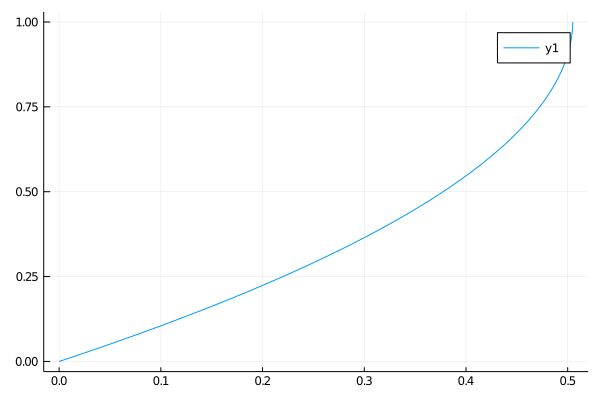
\includegraphics[scale=0.5]{1D_low_res.png}
		
		
	\section{Results: 2D Approach}
	First, we ensured our solution was converging as expected by decreasing $ \Delta z $ by orders of 2, and checking to make sure the error was decreasing at the same rate. This is based on direct solve using CPU.
		\begin{center}
		\renewcommand{\arraystretch}{2.0}
		\begin{tabular}{c|c|c|c}
			\hline\hline
			$\displaystyle \Delta z $&$\displaystyle \varepsilon_{\Delta z} = \sqrt{z}\lVert u-e\rVert $&$ \displaystyle \Delta\varepsilon = \frac{\varepsilon_{2\Delta z}}{\varepsilon_{\Delta z}} $&$\displaystyle r = \log_2\left(\Delta\varepsilon\right) $\\
			\hline
			0.1&$8.02\times 10^{-16}$&Empty Entry&Empty Entry\\
			0.05&$1.8\times 10^{-15}$ &0.446&-1.165\\
			0.025&$4.6\times 10^{-15}$&0.392&-1.351\\
			0.0125&$1.02\times 10^{-14}$&0.452&-1.146\\
			\hline
		\end{tabular}
	\end{center}
	We timed the two-dimensional problem using the four methods listed above and depict the results in the table below for \Delta z = 0.01. We did not do direct solve on GPU.
	\begin{center}
		\renewcommand{\arraystretch}{1.5}
		\begin{tabular}{c|c|c|c}
			\hline\hline
			\textbf{Device}&\textbf{Method}&\textbf{Time [s]}&\textbf{Error~~$\sqrt{z}\lVert u-e\rVert $}\\
			\hline
			\multirow{2}{*}{CPU}&Direct&0.027&$1.31\times 10^{-14}$\\
			&CG&0.025&$1.49\times 10^{-10}$\\
			\hline
			\multirow{2}{*}{GPU}&Direct&N/A&N/A\\
			&CG&0.2&$1.49\times 10^{-10}$\\
			\hline
		\end{tabular}
	\end{center}
	
	Here is the graph for 2D low res:\\
	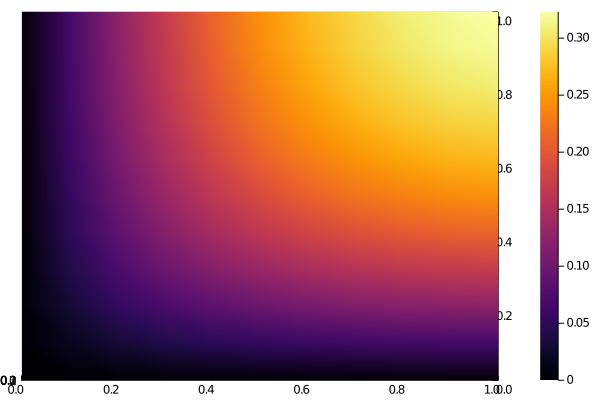
\includegraphics[scale=0.5]{2D_low_res.png}
	
	Here is the graph for 2D middle res:\\
	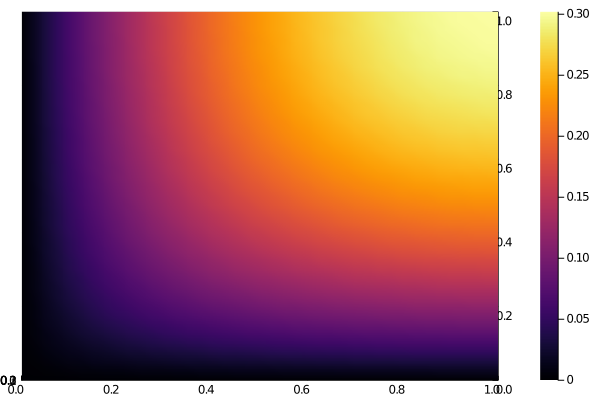
\includegraphics[scale=0.5]{2D_mid_res.png}
	
	Here is the graph for 1D high res:\\
	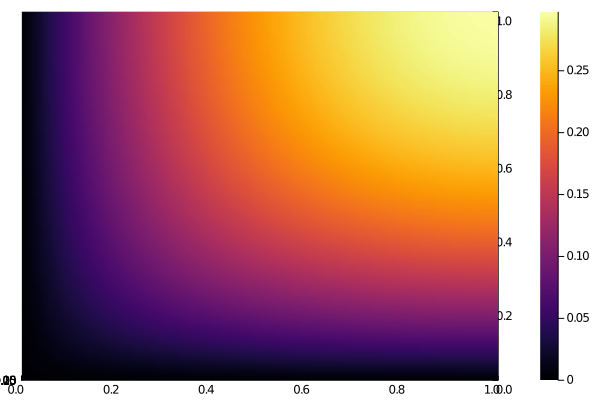
\includegraphics[scale=0.5]{2D_high_res.png}
	
	We can see it is working based on the graph changes from low res to high res.
	
	\section{Code Listing}
	The code we wrote is attached below
	\begin{lstlisting}

	\end{lstlisting}
\end{document}